% REMEMBER: You must not plagiarise anything in your report. Be extremely careful.
%
% We give thanks to the Gods of LaTeX, who in their eternal graciousness, 
% have granted that this document may compile without errors or overfull hboxes.

\documentclass{l4proj}
    
%
% put any additional packages here
\usepackage{pdfpages}
%
\newcommand{\pdfsection}[2]{\includepdf[pages=1,pagecommand={\section{#1} }, width=0.75\textheight]{#2}
\includepdf[pages=2-,pagecommand={}, width=0.75\textheight]{#2}}

\newcommand{\pdfpage}[2]{\includepdf[pages=1,pagecommand={\section{#1} }, width=0.80\textheight]{#2}}


\begin{document}

%==============================================================================
%% METADATA
\title{Making Projects: Dynamic Project Syllabuses for People with Intellectual Disabilities}
\author{Claire Williamson}
%\date{March 24, 2023}

\maketitle

%==============================================================================
%% ABSTRACT
\begin{abstract} 
    Inaccessible instructions and lack of knowledge of the needs of people with disabilities are two barriers preventing disabled people, especially people with intellectual disabilities, from participating in tangible learning. We designed and evaluated "Making Projects", a new software tool that adapts tangible learning project tutorials to suit users' needs by creating a customised syllabus of project tutorials. We explored the challenges people in this area of tangible learning have reported, and attempted to understand their impact on our projects and therefore how to build pathways through them to allow people with disabilities to develop strategies to overcome these challenges. We evaluated it one-on-one with three participants who had relevant experience with tangible learning and people with disabilities, in a lab study consisting of interviews and engagement with the tool.  This revealed that participants found the tool intuitive, useful, and accessible for people with intellectual disabilities.   

\end{abstract}

%==============================================================================

% EDUCATION REUSE CONSENT FORM
% If you consent to your project being shown to future students for educational purposes
% then insert your name and the date below to  sign the education use form that appears in the front of the document. 
% You must explicitly give consent if you wish to do so.
% If you sign, your project may be included in the Hall of Fame if it scores particularly highly.
%
% Please note that you are under no obligation to sign 
% this declaration, but doing so would help future students.
%
\def\consentname {Claire Williamson} % your full name
\def\consentdate {24 March 2023} % the date you agree
%
\educationalconsent


%==============================================================================
\tableofcontents

%==============================================================================
%% Notes on formatting
%==============================================================================
% The first page, abstract and table of contents are numbered using Roman numerals and are not
% included in the page count. 
%
% From now on pages are numbered
% using Arabic numerals. Therefore, immediately after the first call to \chapter we need the call
% \pagenumbering{arabic} and this should be called once only in the document. 
%
% Do not alter the bibliography style.
%
% The first Chapter should then be on page 1. You are allowed 40 pages for a 40 credit project and 30 pages for a 
% 20 credit report. This includes everything numbered in Arabic numerals (excluding front matter) up
% to but excluding the appendices and bibliography.
%
% You must not alter text size (it is currently 10pt) or alter margins or spacing.
%
%
%==================================================================================================================================
\chapter{Introduction}
\label{introduction}

% reset page numbering. Don't remove this!
\pagenumbering{arabic} 
This chapter shall outline the motivations for making tangible learning more accessible for people with disabilities, and will present the aim of this project along with the related objective. We will also introduce a user story, which will be continued throughout as a way of putting this project into context. 

\section{Motivation}
Tangible learning is simply the concept of learning by using physical objects. It has been found to be useful in teaching computer science-related concepts among others \citep{Mar2015}, and can provide an effective and engaging alternative for education, especially for people whom traditional learning is not well suited for. Tangible learning can take many forms but of particular interest to this project are those that utilise technology. This includes electronics and robotics tool kits, digital fabrication, and tutorials for these accessible via the Internet. Technology can be used to enhance tangible learning, make it more accessible to a wider group of people, or carry it out in its entirety \citep{Qi2018}.

One group that could benefit from tangible learning are people with disabilities, specifically people with intellectual disabilities and other cognitive impairments. Intellectual disabilities are a group of neurodevelopmental disorders which greatly affect a person's mental ability, commonly affecting functions such as problem-solving, abstract thinking, and learning. These in turn cause impaired social and cognitive functioning, for example in memory, attention, and communication. \citep{Ame2013} 
In an increasingly digital world, disabled people on average have less digital literacy \citep{Llo2022}. Therefore it is important to find effective ways of educating - not just in teaching of computer science concepts, but by creating technology for carrying out that education. Tangible learning offers us a way to do so. 

However, the current state of tangible learning remains inaccessible to many people with disabilities, especially people with reduced cognitive functioning \citep{Seo2019}. Many factors can contribute to this, such as the equipment are required being physically inaccessible. This could be due to them being specialised tools that average person does not own, or public workshops with these tools not being accessible for disabled people. There is also the issue of the tools requiring high levels of manual dexterity or vision, for example small buttons or screws. People with knowledge of working with people with disabilities often don’t have knowledge of the tools and technology, and vice versa, leading to a knowledge gap \citep{Raj2015}. Resources which could bridge this gap fall short - tutorials are frequently written with complex technical language, unclear and confusing instructions, assumptions about the person's ability, and in inaccessible formats.

Attempts have been made to lower these barriers and get people with disabilities involved with tangible learning. They have highlighted a need for adaptable resources that can be used in various situations, as well as expansion into including more complex projects to allow people to continue their learning journey. As people with disabilities gain more experience in tangible learning, they can develop strategies to overcome and address the constraints, challenges and difficulties they face whilst carrying out tangible learning projects.

This highlights the need of accessible tangible learning not just for introducing new concepts and learning opportunities for people with disabilities but also as a way to continue this learning in a way that suits them.

\section{Aim}
We propose Making Projects, a new tool which sorts tangible learning project tutorials dynamically based on an individual users needs. This is so that people with disabilities, specifically intellectual disabilities, can access the benefits of tangible learning. It aims to create a personalised syllabus of project tutorials so that the user can improve their knowledge and skills through a guided path. 

\section{Objectives}
In order to achieve this aim, we have defined the following objectives:
\begin{itemize}
    \item Create a process for capturing the requirements of the user in relation to tangible learning projects, in an accurate and accessible way.
    \item Design and implement an algorithm which dynamically creates a syllabus of project tutorials for an individual user. 
    \item Design and implement a method and structure of displaying project tutorials in a way that is adaptable and accessible. 
    \item Evaluate the tool with people who have knowledge of the area of tangible learning and people with disabilities. 
\end{itemize}

\section{User Story}
In order to give a better understanding of the tool, we have created a user story which outlines a potential usage situation of Making Projects. We will return to it at relevant sections in order to illustrate what is occurring and why. \\


\noindent{\setlength{\fboxsep}{1em}\fbox{%
    \parbox{\textwidth-2em}{% 
    Ruby is a volunteer at her local disability support charity in Glasgow. She goes to their meetings twice a week for three hours, and spends time with a group of four people that are living with various intellectual disabilities. She spends this time trying to find activities to entertain and interest them. Ruby is keen to help the group to engage with science and technology more, but currently finds this difficult because she is a graphic designer and does not know much about science. She has tried to look up STEM activities online but has found all of them unsuitable for her group's needs. When they tried to follow one in the past, they found it was unsuitable halfway through and that they were not able to continue it. This led to her group feeling frustrated and not wanting to do any more of these activities. 
    \\ \\
    With the Making Projects tool, she can describe the barriers each of the people she works with faces and get projects for them that they are able to do. 
    } % 
    } }

%==================================================================================================================================
\chapter{Background}
\label{background}
This chapter discusses relevant research which has formed the background of this project, firstly by looking at the current state of tangible learning and its interaction with people with disabilities. Then we will look at relevant design ideas for creating accessible objects, and prior work that involves bringing tangible learning to people with intellectual disabilities. 

\section{Making and Makerspaces}
The preeminent form of tangible learning is the subculture of ‘making’, which has rapidly grown in both popularity and research interest. Making is centred around ‘makerspaces’ which are workshops accessible to the public. The number of makerspaces, or similar community workshops, in the UK has increased from only a few to almost a hundred in the past decade \citep{Sle2015}, showing that more people are getting involved with them as well as making them available to a wider range of potential users. These makerspaces allow for a sharing of tools and knowledge between ‘makers’ while they carry out their projects. Making is simply the process of physically creating something yourself. More than this, it’s become part of a global movement which champions this process over any end product. \cite{Kuz2010} highlights the benefits “doing it yourself” brings: increasing skills with the tools used, understanding the technological and engineering concepts behind them, and the community aspect created from doing these projects alongside other people.

While traditional workshops are centred around woodworking and metalwork, makerspaces are notably different in their approach which focuses on technology, programming, and digital fabrication. This allows users to learn computing science concepts through the process of constructing and creating projects, as opposed to more traditional methods that require a lot of abstract thought and understanding \citep{Mar2015}.

\cite{Tan2013} notes makerspaces as being sites of innovation, due to the fact that they allow more people the opportunity to design and quickly prototype new ideas. They allow more people from a variety of typically underrepresented demographics the opportunity to create their own products. This leads to a democratisation of product design, whereby the ability to design and make products is no longer solely limited to large companies. They allow people to create products that they personally want and need, and to easily modify the design to further suit them with the use of quick prototyping with digital fabrication tools. 

One area that could benefit from this innovation is DIY-AT. The term Assistive Technology (AT) encompasses a wide range of devices that have the purpose of supporting people with disabilities and allowing them to function better. These could be items as simple as grips for cutlery, walkers, and grab rails, or high-tech devices such as hearing aids and motorised wheelchairs.

However, \cite{Phi1993} finds that AT is regularly unused or abandoned by users. The reasons for this include: 
\begin{itemize}
    \item The user's opinion has not been considered during the selection, leading to a device that is not suitable for their needs or that they don’t want to use.
    \item Devices, especially ones that are most effective for an individual, are difficult to obtain. This can be due to lengthy referral processes and/or the large financial cost.
    \item They do not perform well in the tasks required by the user.
    \item Disability and impairments are fluid in that they affect the person in different ways, often in a short span of time. This means that AT is no longer functional when the user’s needs change, and the AT cannot adapt to this.     
\end{itemize}   

A few different ways have been proposed on how to improve continued AT use. One point is involving the end user more in both the design of technology, and the selection of it. One way this can be done is by “do-it-yourself” AT (DIY-AT). This allows the user more control over the design, resulting in AT that fits their personal needs.  It can also be a more cost effective solution. This is important as traditional AT can be incredibly costly, especially when you take into consideration the fact that people with disabilities tend to earn less money \citep{Off2022}, have higher unemployment rates \citep{Dep2022}, and have additional expenses associated with having a disability \citep{Joh2019}.  

Makerspaces offer an ideal environment for creating DIY-AT, which has been applied in practice. At the same time, there has tended to be a focus on non-disabled people designing and creating the AT which can lead to the same issues listed above. \cite{Hoo2014} states that care must be taken to involve the person with the disability as much as possible in order to create a product that is of use to them.  

\cite{Tay2016} found that in addition to makerspaces being a site for peer learning and innovation, makerspaces function as places that support the well being of their users. They also have the ability to serve the needs of the community in which they are situated, provide spaces for socialisation, and work to reach out to groups that are excluded from such spaces. In the context of Making Projects, these features are particularly advantageous. People living with intellectual disabilities are more likely to feel lonely than people without the disability \citep{Ale2018}. Makerspaces therefore offer a space for them to connect with others and grow their social bonds.

Therefore, makerspaces seem to provide an ideal setting for tangible learning. Makers don’t have the costly overhead of buying their own tools, and are surrounded by like-minded people willing to share their experience. These are factors which could greatly contribute to the breaking down of the aforementioned social and financial barriers that people with disabilities can face. 

Despite this ideology of inclusivity and the motto of “anyone can make”, many makerspaces and making as a whole have issues with what groups are included. There is a disproportionate number of makerspace users that are affluent, non-disabled, white men with a STEM background \citep{Mak2013}. This lack of diversity by itself can discourage members of these underrepresented groups from accessing such spaces. 

Many efforts have been made to lessen this disparity for various groups, to some success. \cite{Qi2018} looked at how their paper electronics toolkit engaged new groups and found that, similar to the e-textile community \citep{Bue2010}, paper electronics offers new ways to include groups in making. This shows that different forms of making can be utilised to effectively engage different demographics of people.


\section{Designing for People with Disabilities}
An important question raised for Making Projects is how to best design something for people with disabilities. In this section we will define and explain several concepts which are relevant to Making Projects.

\subsection{Social Model of Disability}
Central to how to design for people with disabilities is how we think about disabled people and the concept of disability. The social model of disability puts forward the idea that disability arises from situations where society has failed to meet the needs of such people, rather than from any limitations of an individual person \citep{Oli1990}. These barriers can be removed by designing in such a way that disabled people can have equal access, therefore making their disability negligible in this situation. It is in contrast to the medical model of disability, which instead considers disability an issue individual to the person and focuses on individual treatment and intervention. The emphasis is put on the medical implications, rather than the way the person with a disability interacts with society. 

\subsection{Participatory Design}
Participatory design is centred around the concept of fully involving the end user in the design of the product \citep{Per2015} This allows the product to meet their needs and be usable by them. Many designs are inaccessible purely because the needs and requirements of disabled people have not been considered. It aims to combine the knowledge of the development team and the user, to create a better product. This concept ties in well with the culture of making, as a lot of the time the person creating the object has a lot of creative control over the outcome. It is also important for Making Projects, as a tool that is to be used by disabled people and so should be designed with their needs in mind to the greatest extent possible. 

\subsection{Universal Design}
Arguably the most popular design term when designing for people with disabilities, as well as in general inclusive design. With the term first coined in 1985, universal design prioritises designing something which can be used by as many people as possible. This is further defined as “the design of products and environments to be usable by all people, to the greatest extent possible, without the need for adaptation or specialized design.” \cite{Cen1997} 
Its aim is to remove as many potential barriers as possible by taking a wider look at these issues, rather than just individually tackling each barrier. This links nicely to the social model of disability, in thinking about issues on a wider societal scale. 
In order to further explain this concept, the Center for Universal Design outlines seven principles: 
\begin{itemize}
    \item 
Equitable Use: The design is useful and marketable to people with diverse abilities. 
\item
Flexibility in Use: The design accommodates a wide range of individual preferences and abilities. 
\item
Simple and Intuitive Use: Use of the design is easy to understand, regardless of the user’s experience, knowledge, language skills or current concentration level. 
\item
Perceptible Information: The design communicates necessary information effectively to the user, regardless of ambient conditions or the user’s sensory abilities. 
\item
Tolerance for Error: The design minimises hazards and the adverse consequences of accidental or unintended actions. 
\item
Low Physical Effort: The design can be used efficiently and comfortably and with a minimum of fatigue. 
\item
Size and Space for Approach and Use: Appropriate size and space are provided for approach, reach, manipulation and use regardless of the user’s body size, posture or mobility.
\end{itemize}

\subsection{Ability-Based Design}
Universal design and similar approaches have their roots in designing physical objects and buildings to be accessible. However, computer software offers a much more flexible and adaptable environment. \cite{Wob2011} introduces ability-based design as a concept that builds off universal design to offer suggestions on how to use the unique properties of technology to design for disabled people. Its core principle is that there should be a focus on what the user can do, rather than what they cannot do. It presents 6 other principles that designers should follow when creating accessible technology, which we will briefly outline and discuss the ones relevant to our current work:
\begin{itemize}
    \item Accountability: any issues with the system performance should be corrected by changing the system, not the user. This reflects the social model of disability in that it is a fault of the system that a user cannot access it, not a fault with the user.
    \item
Adaptation: it’s recommended that the system interface adapts to best fit each user's needs and abilities, either automatically or by the user. This results in a more accessible system, that is tailored to a users needs rather than a "one size fits all" approach which may inadvertently create issues. 
\item
Transparency: the interface may tell the user what adaptations have been made, and allow them to modify them. It's important for the user to have control, as they best know what they need. 
\item
Performance: the system may access the user’s performance and use that data to measure, model, or predict their performance. This can allow for the system to better understand the needs of the user in order to better adapt to them. 
\item
Commodity: it’s encouraged that the system consists of low-cost and readily available hardware and software. This allows for more people to use the system, as there is no cost barrier.
\end{itemize}



\section{Related Work: People with Disabilities Making}
People with disabilities making combines the topics previously discussed. Prior work about people with disabilities, especially intellectual disabilities, carrying out tangible learning has revealed several relevant points. It has also highlighted where further research is needed. That is what we will discuss in this section. 

Many making toolkits and resources are inaccessible to people with intellectual disabilities. This can be due to them requiring complex physical manipulation, relying on the user remembering prior concepts, and/or being in formats that are difficult to understand \citep{Lef2016}. In response to this, accessible tool kits have been developed to facilitate their tangible learning in a way suitable for their needs. 

\cite{Ell2021} developed a making toolkit “TapeBlocks” which incorporated electronics and simple motors. They aimed to lower the barriers for entry to making by creating an electronics toolkit that could function as an initial step into tangible learning/electronics. The core component of TapeBlocks are large foam blocks on which conductive tape is placed. These blocks can then be easily connected together to form different circuits. 
By using these large foam blocks, they lowered the level of fine motor control needed to create circuits, as well as not requiring a lot of physical strength as the foam is lightweight. The components are also affordable, and all these factors lead to their appeal.  

\cite{Sen2022} then built on this work to create an accessible electronics toolkit for people with intellectual disabilities, that offered an increased amount of circuit creation activities. It aimed to lower the physical and cognitive barriers present in other electronics tool kits.

Several key themes have emerged from these works and other similar research: 

\textbf{Instructions:} 

\cite{Boc2022} found that it’s best to not use technical jargon as well as breaking language down and keeping the projects simplified. 

As well as avoiding complex technical language, writing instructions in Plain English can promote independent understanding.  This is because people with cognitive impairments are more likely to understand these instructions on their own, without additional support. 
Having any instructions be available in different formats is important to allow for more people to access them \citep{Bra2014}. This could include having printed large text, digital, and braille format. 

\textbf{Project Considerations:} 

\cite{Bra2014} found that when deciding what types of projects to carry out or offer, consideration should be made of what different abilities the potential users will have. Any changes to the projects that they will need should be carried out in advance. If it is not possible for a project to be adapted, there should be another activity that they are able to do.
Projects that are fully participatory for the user tend to be more successful in terms of interaction and enjoyment. Therefore creating projects that are suitable for someone to do as independently and as fully as possible, as in Making Projects, will improve the user's experience.
Additionally, adults with intellectual disabilities preferred and benefited more from focused group activities. This suggests that carrying out projects in a group environment, such as a makerspace, is well suited to their needs. 
A point often echoed is that participants enjoy personalised projects and getting to create what they want. \cite{Boc2022} This helps foster a sense of independence and control in the participant. The reverse of this is also true, in that it is important for anyone supporting the disabled person to not take control of the situation, and instead allow them to problem solve. 

\cite{Ell2021} puts forward that projects themselves should aim to be affordable, require little barriers for engaging with them, and be able to be experimented with. This echoes similar principles in both universal and ability based design, emphasising the importance of their principles in such work. 

\cite{Hol2014a} found that you can increase a person with intellectual disabilities understanding of how something works by having visual indicators. They modified the design of pre-existing electronics modules to make their functions clearer and easier to understand, as well as making each component look more different to each other. This allowed people with intellectual disabilities to more easily create electronic circuits, as well as having less errors during the process. This highlights the importance of visual design, especially when users may not be able to understand text. 

\cite{Sen2022} suggests that making sessions should aim to be kept short (45-90 minutes) as keeping participants engaged and concentrated is difficult for longer periods of time. This can be achieved with Making Projects, as by having a range of project tutorials, a simpler one can be selected which will take less time to complete. 

\cite{Ell2021} states that the people who used their toolkit expressed an interest in learning and developing their electronics skills further, and wanted to know how to do that. \cite{Sen2022} did this partially by offering more ways to use electronics in an accessible way. This highlights a need for extending these beginner level tool kits to allow users to go further in their learning. However current research and resources are still limited in what extent this can be done, and only focusing on specific areas with tool kits. 

Making Projects aims to build on the principles found in prior research to create a way for people with IDs to start and continue their tangible learning journey, to an open ended, more advanced level. By combining different areas of making projects, such as electronics and robotics, which have been developed through research. 

\section{Related Tutorial Sites}
There are many online resources and websites that have the purpose of sharing tangible learning project tutorials. However, \cite{Wak2015} notes that often these tutorials are not of high quality, leading to difficulties in implementing the projects. This can be due to issues with communication, sequencing of instructions, and the tools used.
This section will provide a review of several of these resources, in order to identify their strengths as well as areas which may be inaccessible to people with intellectual disabilities. It will also discuss how they have influenced the development process and design of Making Projects, and how we aimed to address the areas of inaccessibility that are present in them. This process also served to understand what information our project tutorials should contain in order to be completed successfully by users. For each site, the example tutorial shown was selected by sorting the tutorials by "popularity" and choosing a suitable one. 

\subsection{Thingiverse}
Thingiverse\footnote{https://www.thingiverse.com/} is the largest online community for 3D printing. It is a website that contains over 2.5 million user-uploaded tutorials for 3D printing projects. It allows users to "remix" other people's tutorials, in order to customise them however they wish, and is aimed at people with all levels of experience with 3D printing. In theory, this is ideal for people with intellectual disabilities as there will be projects they can do as a complete beginner, and can then build up to more complex ones. In practice, Thingiverse does not have a way of denoting how complicated a project is, or filtering projects by their difficulty. 

\begin{figure}[htb]
    \centering
    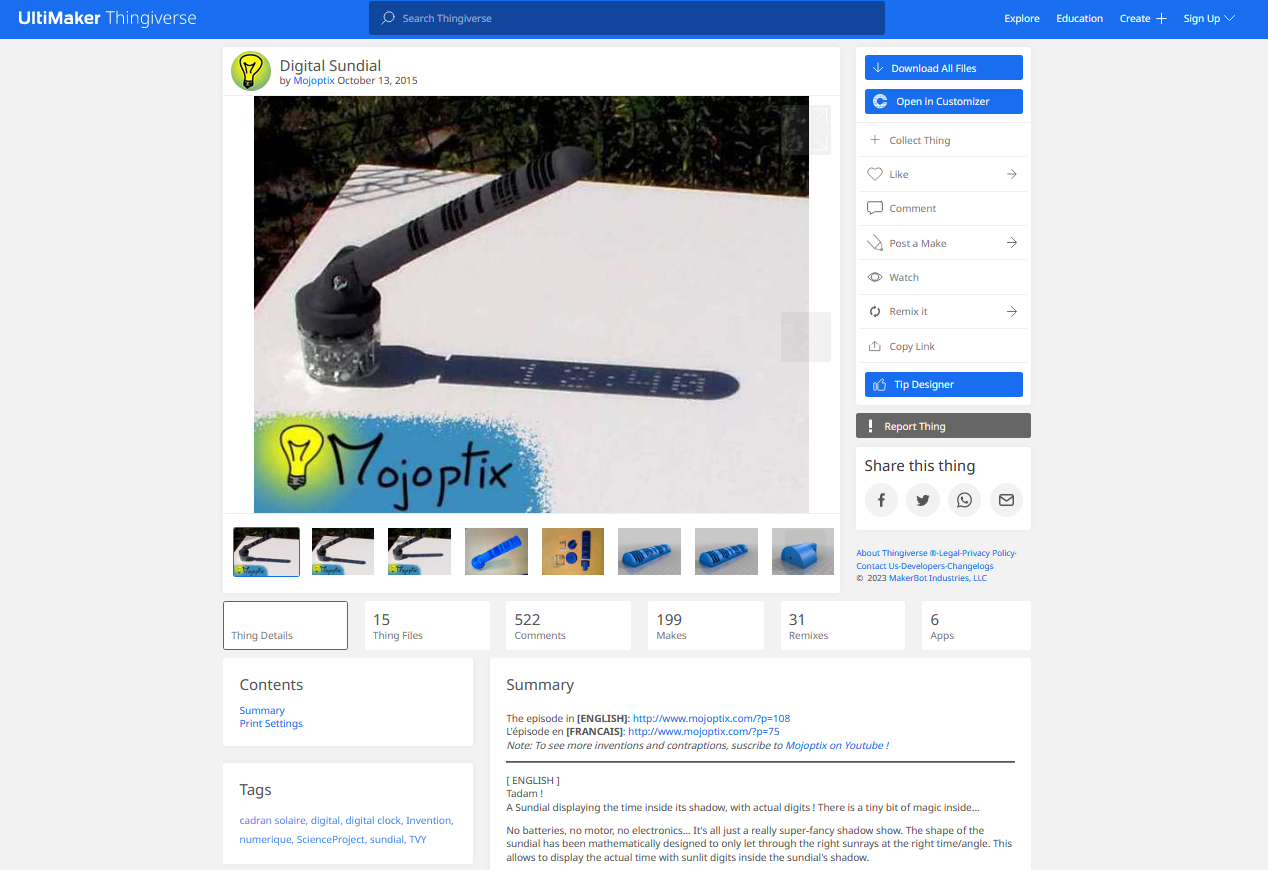
\includegraphics[width=0.75\linewidth]{images/thingiverse.png}    

    \caption{View of a tutorial for a 3D printed sundial on the Thingiverse website.
    }
    \label{fig:thingiverse} 
\end{figure}

By its very nature, Thingiverse is limited in only showing projects that require a 3D printer. The information displayed for each project is relatively limited and gives no indication of what skills the user needs to be able to complete it. This is information that can be particularly important to those with intellectual disabilities to know prior to beginning a project, and its absence could dissuade such users from attempting the projects at all. Despite this lack of project information, the user interface contains a lot of different components which could be easily overwhelming and distracting for a person with intellectual disabilities \citep{Cha2013}. 

\subsection{Make: Projects}
Make: Projects\footnote{https://makeprojects.com/home} is a joint venture between Make:, a company focused around making which publishes the most popular magazine for the making community, and engineering.com, which is a collection of engineering based resources. Similar to Thingiverse, it functions as a space for users to upload and share their project tutorials. However, unlike Thingiverse these projects span across all types of making and DIY. 

\begin{figure}[htb]
    \centering
    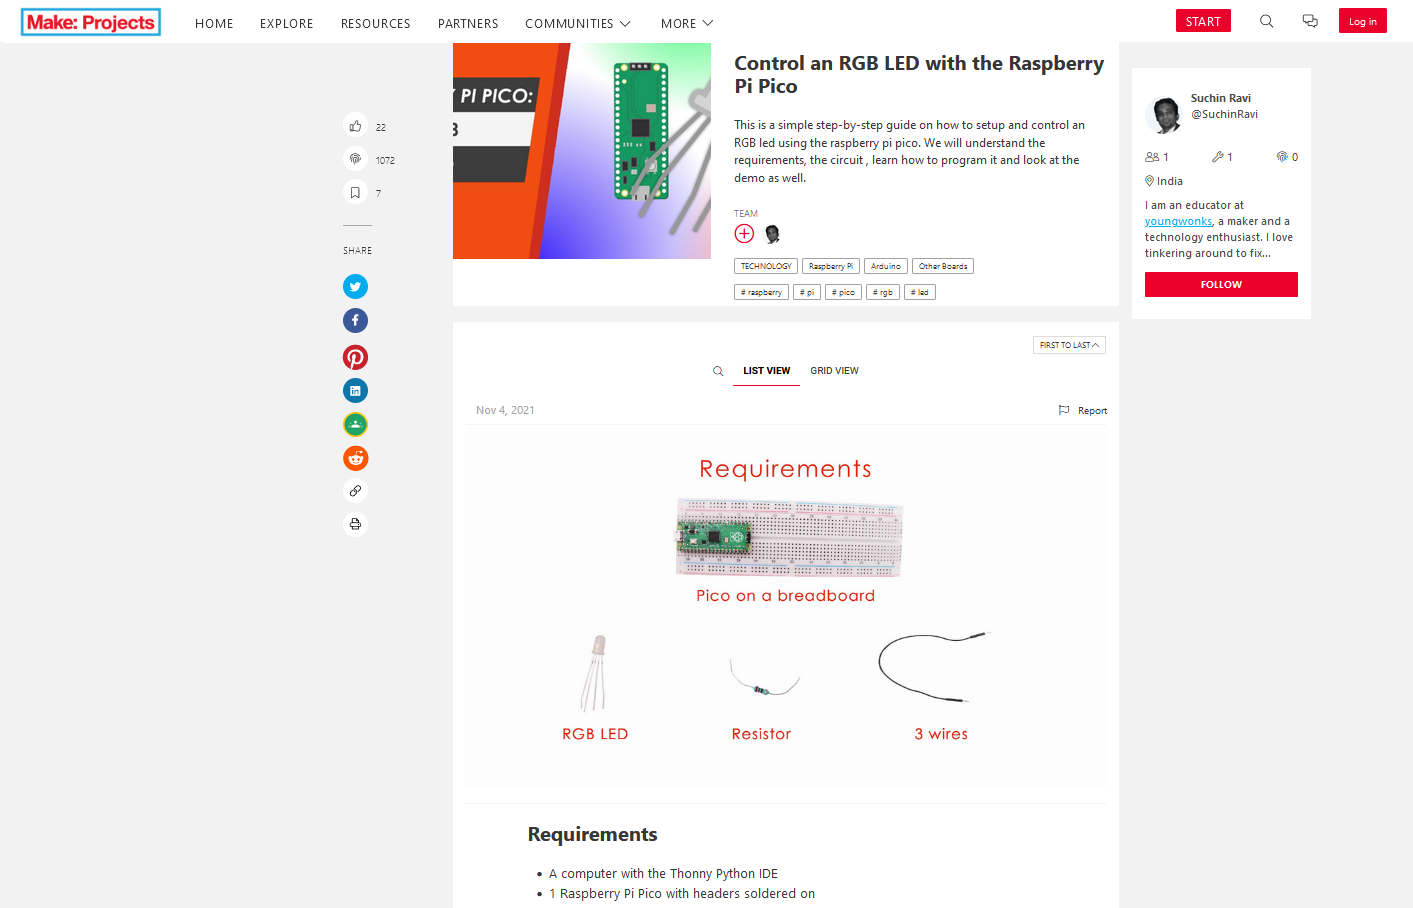
\includegraphics[width=0.75\linewidth]{images/make-projects.png}    

    \caption{View of a tutorial for a LED controller on the Make: Projects website.
    }
    \label{fig:make-projects} 
\end{figure}

It has some identifiers for what a project contains, but these are limited to only the categories of projects. This could make the process of finding suitable and relevant projects a more time consuming task than necessary. Additionally the identifiers are in the form of small, similar looking icons which could cause confusion to a user. It shows less unnecessary information than Thingiverse, but still poses potential distractions. 


\subsection{Autodesk Instructables}
Instructables\footnote{https://www.instructables.com} is another site containing project tutorials. It is part of Autodesk which is a large software corporation with a focus on software for manufacturing. Similar to Make: Projects, Instructables attempts to cover a wide a range of projects as possible. 
\clearpage 
\begin{figure}[htb]
    \centering
    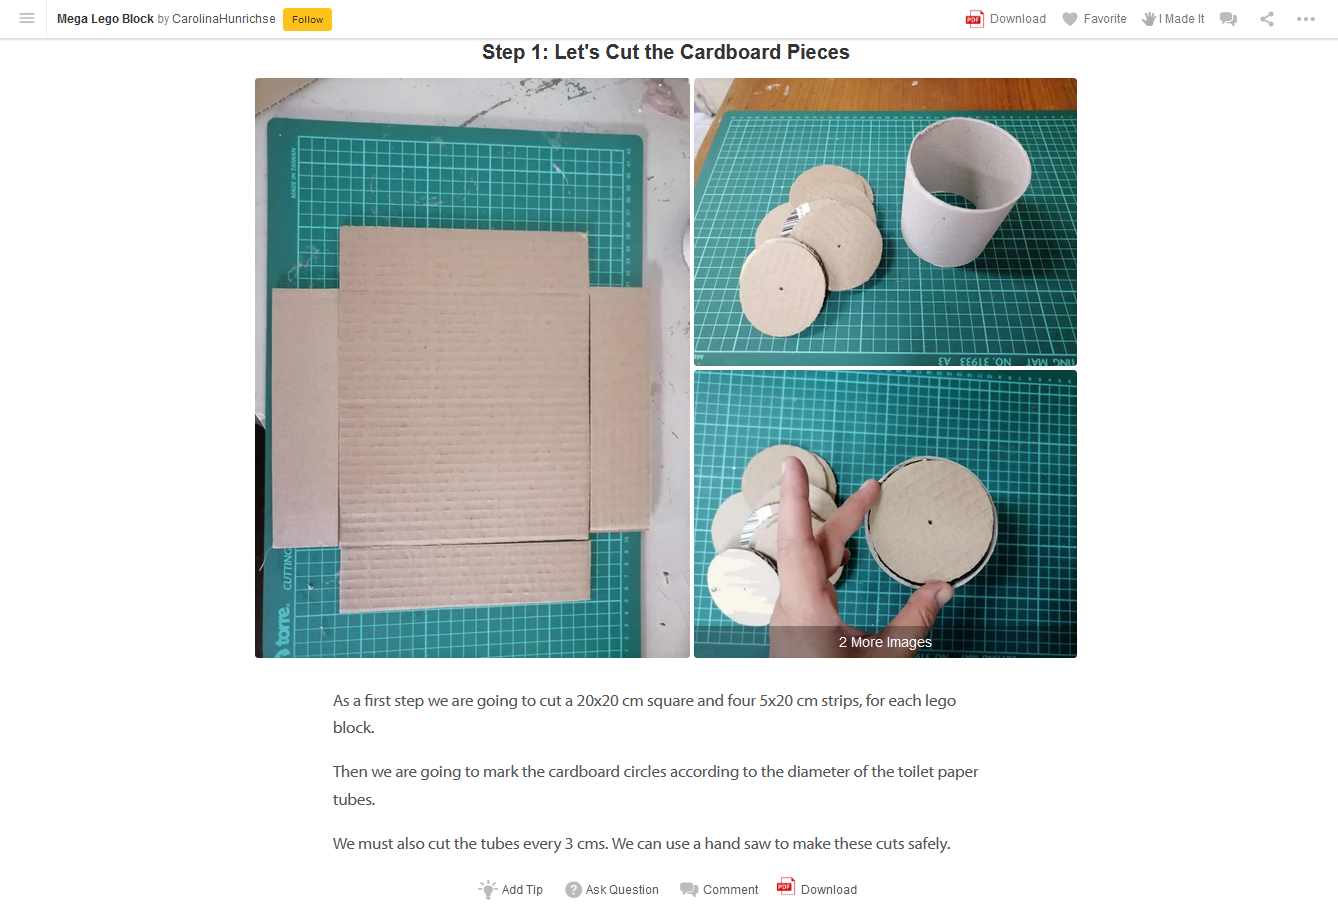
\includegraphics[width=0.75\linewidth]{images/instructables.png}    

    \caption{View of a tutorial for a cardboard Lego block on the Instructables website.
    }
    \label{fig:instructables} 
\end{figure}

Out of the three resources discussed here, it has the most simplified user interface for the project tutorials. It focuses purely on the instructions and information needed to carry out the project. However, it has no filtering by or communication of project difficulty. Like with the other resources, the quality of the tutorials is dependant on the individual uploader which can lead to inconsistency. This can cause problems for all people attempting to complete this projects \citep{Wak2015}, but these problems will be further intensified for people with intellectual disabilities. 

%==================================================================================================================================
\chapter{Requirements Analysis}
\label{requirements-analysis}
This chapter will discuss what Making Projects needs to have in order to fulfil its aims, in the form of its functional and non-functional requirements. These requirements were drawn from the points discussed in chapter \ref{background}, in addition to the following analysis of the project's stakeholders. 

\section{Stakeholders}
From the above methods we identified various stakeholders and what their needs in this situation would be. This gave us a better idea of what the tool should do and how it should do it. The stakeholders we identified were:
\begin{itemize}
    \item Target users: the people with disabilities themselves. They wish to learn more about tangible learning, and carry out projects that interest them. They may have a diverse range of impairments. 
    \item Their supporters: people who would be coming into the space with the target user in order to assist them. These are people such as professional and family carers, and educators. They may not have any technical knowledge of tangible learning. 
    \item Tangible learning experts: people who would already be in the space that have knowledge of making, and who are interested in helping others enter that space. These are people such as other makerspace users, instructors, and owners. They may not have much knowledge of working with people with disabilities and the challenges they would face in this situation.
    \item Disability advocates: professionals that would like to help more people with disabilities to engage with tangible learning. This includes disability support organisations, disability rights advocates, and medical professionals. They may wish to use the tool as a resource they can signpost people to. 
\end{itemize}


\section{Functional Requirements}
These functional requirements detail specific behaviours and functions of the tool that will allow it to reach the aims discussed in chapter \ref{introduction} These requirements are prioritised with the MoSCoW method, which gives an indication of how important a feature is to the final product achieving its goals. The requirements are also given itemised codes and titles, in order to be able to easily refer to them throughout the project. These itemised codes also reflect the level of priority the requirement has, and that it is a functional requirement. 

\subsection{Must Have}
These are features that the tool needs to have in order to meet the aims given in chapter \ref{introduction}. 

\textbf{FR-MH-1} Project Tutorials: The tool must allow users to view various making project tutorials. The tool adapts the tutorials it shows in order to meet the user's needs. Users can clearly see if a project meets their requirements. The user does not have to log in or create an account to view them. This will allow people with disabilities to get project tutorials that are accessible to them, in order to carry them out and gain the benefits of tangible learning. 

\textbf{FR-MH-2} User Accounts: Users can easily register for an account with the tool. 

\textbf{FR-MH-3} Information on Skill Areas: Logged in users can tell the tool what their current skill level in various areas is. The areas will be relevant to the types of projects, as well as common barriers people with intellectual disabilities face in tangible learning. Users should be able to clearly tell what effect their information has, and can easily change it. 

\textbf{FR-MH-4} Physical Tools Used for Making: Users can input what physical tools they have access to and their current experience level with that tool. Similarly, the project tutorials will state what physical tools are required for that project and the level of experience needed. 

\textbf{FR-MH-5} Syllabus: Once a user has logged in and given their information on skill areas and physical tools, the tool must allow them to create a syllabus. The user specifies a project tutorial that they want to be able to do, and the tool will create a path of projects which the user can follow to gain the skills needed for their selected project. \\

\noindent{\setlength{\fboxsep}{1em}\fbox{%
    \parbox{\textwidth-2em}{% 
Ruby works with four people: Cody, Rex, Kira and Deanna. Deanna has problems with her physical coordination, and has poor eyesight, which makes doing tasks such as screwing small electronic components very difficult for her. However, through the process of working through a Making Projects syllabus, she works out ways to make this easier. One way she does this is by placing any components on a white background and using a magnifying glass so that she can more clearly see them. This allows her to work through the projects, perhaps at a slower pace, but she can still complete it. 
    } % 
} }

\subsection{Should Have}
These requirements are not essential but are important aspects in creating a functional tool.

\textbf{FR-SH-6} Record of Project Completion: logged in users can indicate when they have completed a specific project. If the project is in their syllabus, then a progress bar can be displayed. The user's profile can display what projects they have completed. 


\subsection{Could Have}
The following requirements are not needed to meet the aims of Making Projects but would improve the user's experience with it. These are also potential areas of future work, as the current project has a limited time frame. 

\textbf{FR-CH-7} Guide for Project Adaptation: the tool contains a guide on how to adapt project tutorials to make them more accessible for people with disabilities. This could then be used by people with existing tutorials in order to make them more accessible. It could also be used alongside the creation of new tutorials to ensure that they are suitable. 

\textbf{FR-CH-8} Dynamic Project Tutorials: Having a single project being adaptable so that users with different requirements can complete it. 

\textbf{FR-CH-9} DIY-AT Project Tutorials: the tool contains project tutorials that involve creating a piece of DIY Assistive Technology, which could allow the person to more easily complete other making projects as well as improving their general day-to-day functioning. 

\section{Non-Functional Requirements}
These non-functional requirements specify general properties of the tool. As with the functional requirements, they are prioritised using the MoSCoW method and itemised accordingly.  

\subsection{Must Have}
These are aspects which the tool must have in order for it to meet its aims. 

\textbf{NR-MH-10} Ability Based Design: The tool must follow the principles of ability-based design as discussed in chapter \ref{background}. It must focus on what a user can do, rather than what they cannot do.

\textbf{NR-MH-11} Universal Design: The tool is able to be effectively used by a wide a range of people as possible, and follows universal design guidelines where feasible. This includes considerations such as making content accessible to screen readers, and using clear language.

\textbf{NR-MH-12} Freedom of Choice: Users have freedom to choose what projects they would like to do. 

\textbf{NR-MH-13} Extensibility: The tool is created in such a way that is is easy to add new components, without having to alter pre-existing code. 

\textbf{NR-MH-14} Maintainability: The tool's code base, as well as the tool as a whole, is designed and well documented so that others can readily continue working on it. 

\subsection{Should Have}
These are aspects which would greatly improve the design of the tool, but are not necessary for a successful project. 

\textbf{NR-SH-15} Embedded Tutorials: Project tutorials should be in a simple format so that they can easily be embedded in other sites.

\textbf{NR-SH-16} Participatory Design: The design and development of the tool is based on the real experience of the intended end users. The end users should be involved to the highest level possible. 

%==================================================================================================================================
\chapter{Design}
\label{design}
This chapter will discuss the final design of the tool, beginning with an overview and then looking at specific key elements. It will detail important design choices, along with their justification and the relevant requirements they aim to meet. 

Making Projects underwent a major refactor halfway through. Important changes from which are highlighted in the relevant sections in both the design and implementation chapters. This refactor was due to the project specification evolving as we got a better idea of what the tool should do, and allowed for components to be more effectively designed and more clearly separated. 

\section{Overview of Making Projects}
The Making Projects tool will consist of a library of making project tutorials that can be adapted to an individuals specific needs. As well as these individual projects, the tool can create a customised syllabus of projects for a user, in order to create a path towards their specified goal. The user will tell the tool their needs, which it will use to make the adaptions resulting in projects and syllabuses which that user is able to complete.  

The system structure for this can be described using the Model-View-Controller architecture. In which the user makes requests through the view (the user interface), which then sends this request to the controller to determine the appropriate action. In some cases this action requires the controller to query specific data from the model (in our situation, this is a database). It then processes this data to return a response to the user. 
\begin{figure}[htb]
    \centering
    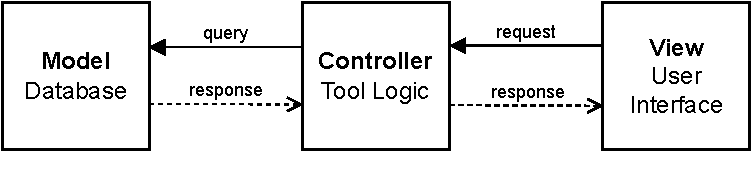
\includegraphics[width=0.75\linewidth]{images/MVC.pdf}    

    \caption{Model-View-Controller Architecture Diagram.
    }
    \label{fig:MCV_fig} 
\end{figure}

\section{Syllabus of Project Tutorials}
The main feature of the tool is the automated syllabus creation. Its purpose is to allow the user to build up their skills in manageable steps so that they are able to complete a project of their choosing. 

\subsection{Syllabus Creation}
The design of the syllabus creation is as follows. 
\begin{algorithm}
\While{end project requirements > profile requirements}{
    Find what skills to improve\;
    Find a project with an improved skill\;
    Add that project to syllabus\;
    Update the profile's requirements\;
}
\end{algorithm}  

Firstly, the user interface asks the user to choose what project they want to be able to do. It sends this request to the controller, which queries the database for the information on that project. This information includes specifics regarding what skill levels are needed to successfully carry out this project, as well as the physical tools. 

Making Projects then queries the database for the user's information, which will contain information in a similar structure to that of the project tutorial. It compares the skill level information of the project with that of the user. If the user already has suitable skills to carry out this project, then the syllabus will only contain the chosen project.

In most cases, the user won't already have the skills needed. In that situation, the controller calculates what areas they need improve. Then it goes through each of these areas, and attempts to find a suitable project tutorial. This is a project which has identical skill area levels to that of the user, apart from in the specified area for improvement whose level will be increased by one. If no project tutorial can be found matching those requirements, it repeats this process with the next skill area and so on. If no project is found for any of these skill areas needing improvement, it repeats the search process for each area but with the conditions that all other skill area's can be equal to or less than the user's current profile values. This increases the chance that a complete syllabus can be created, without needing projects with every combination of skill requirement values.  

Once a project is found, it is added to the syllabus. The user's skill area requirements are then updated to reflect this project i.e. the value of one skill area will increase by one. Then this entire process will repeat until the user has all the skill levels needed to carry out their end project. At that point, the end project will be added to the syllabus, and the syllabus as a whole will be presented to the user. 

\subsection{Syllabus Design Considerations}
The original syllabus design was that there would only be three or four set syllabuses that a user could choose from. This idea was changed so that the end project choice could be completely customised by the user. This is important in meeting the requirement \textbf{NR-MH-12}, in allowing the user to make their own choices. It also allows for more flexibility of the system, as with the final design it is still possible to have set syllabuses but not the other way around. 

Another design consideration is that of the granularity of the skill levels. In other words, the jump in difficulty between each value, and the total range of values for a skill. We decided on an initial range of 1-3 for each skill area, which is discussed further in section \ref{design-skill-area}. If the jump between difficulty levels was found to be too great, greater granularity could be added, or multiple projects with that same difficulty could be added to the syllabus before one with that increased level.  

\section{Skill Area Requirements}
\label{design-skill-area}
Another key area which is involved in a many areas of the tool is that of the skill area requirements. These are common skills present in tangible learning projects, and which people with disabilities struggle with. They are used to categorise the needs of both users and projects in regards to these areas.

It is important for the tool to have a way of accurately gauging both what a user can do, and what is needed on behalf of the user to complete a project.

\subsection{Structure}
This information was further split up into abstract skills, and physical tools used for projects. 

The skill areas we chose to focus on are drawn from the relevant literature as ones which people with intellectual disabilities and other cognitive impairments have issues with, especially in the context of tangible learning. We decided to select four of these areas for our initial tool, but additional area's can be easily added or changed. The areas which we selected are as follows: 

Dexterity: The physical motor skills needed for tangible learning projects can be a pivotal barrier. People with intellectual disabilities commonly have motor impairments. Clearly stating what level of manual dexterity is needed to complete a project will allow both the tool and the user to gauge if they can complete a project. 

Language: As discussed, issues with instructions are prominent. As well as having all instructions be clear, having more complex language in instructions allows for more advanced projects. There is a need for flagging what complexity of language is used in a project. Additionally, the use of images alongside text can be used by people who may not be able to understand written language, as well as improving the understanding of those who do. 

Memory: Many tutorials make assumptions about the users cognitive load, which is how many concepts a person can remember. People with intellectual disabilities typically have reduced functioning in this area. For example, project tutorials that signal that they are suitable for people with a lower cognitive load may explain relevant concepts frequently before a user needs to apply them.

Vision: A persons level of vision can have a large affect on how they can access tutorials and the actual physical process of making. Therefore it is important to make clear how difficult a project is in this area. 

\subsection{Elicitation from User} 
The process of getting these requirements from the user is important. Accurately understanding the needs of a user is difficult for both the tool and the person. To make this process as simple and effective as possible we designed a form for the user to select what their needs are. We wished for this form to focus on what the user was able to do (in keeping with \textbf{NR-MH-10}), and so it contains a series of statements that explain what a person can do and the corresponding skill level for that ability. 
It was also crucial to have clear examples for each skill level, rather than abstract concepts that could be difficult to understand. 
In following with the ability-based design principles \citep{Wob2011}, we also needed the impact of these requirements to be clear to the user, as well as being easily updated or modified by them. \\

\noindent{\setlength{\fboxsep}{1em}\fbox{%
    \parbox{\textwidth-2em}{% 
Ruby's group's are all affected by their intellectual disabilities in different ways, and to different extents. When Ruby wants to find an activity that they can do, she has to consider each person's individual needs which can get confusing. Often she ends up with activities that her group are not really interested in doing. 
With Making Projects, she can support each person in figuring out what are they able to do, which they can then use to see if projects are suitable for them. 
For example, she can sit down with Cody and work out that since he has poor physical coordination he has the equivalent “low” dexterity level on Making Projects. Likewise, he does not have impaired vision so his vision level is “high”, and so on for each skill area. 


    } % 
} }



\section{Project Tutorials}
The content of the projects themselves will mostly be taken from various online sites, covered under Creative Commons licence, and manually adapted by us to follow these guidelines which are drawn from chapter \ref{background}. 
\begin{itemize}
    \item All written text is as near as possible to being in plain English. Writing in plain English is a learned skill which requires experience, and we were unable to dedicate the time to doing so. However it provided a logical point to aspire to when writing text for the project.
    \item Instructions consist of clear numbered steps. This allows users to easily see the order of what they have to do, as well as helping in the troubleshooting process by outside parties. 
    \item The format was easy for screen readers to process. While we aimed for the entire tool to be suitable for screen reader technology, a particular focus was placed on the project tutorials as the main feature of the tool. 
\end{itemize}
We also had to process what skill area levels were appropriate for each project. 
The types of projects selected focus on various technological concepts such as digital fabrication, electronics, and robotics. They will also cover various levels of complexity in regards to their skill area requirements. This will allow a larger proportion of users to have project tutorials they are able to do. 
The actual project tutorials themselves were not the main focus of this project, and so they may not be completely accurate. Instead, focus was put on the general structure of the project tutorials and their interaction with the tool. 

The project tutorials interact with the users information to display if they are at a suitable level. Users do not have to be logged in to view projects, as we wish for them to be accessed by the widest range of people and situations.


\section{User Account}
Users can register and log in to the tool. This allows for a users data to persist over several sessions, so that they can gain the benefits from continued use. This also removes the extra time taken to go through the process of entering skill area requirements every time - which could require considerable effort for a person with an intellectual disability. Additionally it removes the burden from the user of remembering their skill area requirement values. 
We wished for the information that needed to be remembered by the user to be as minimal as possible, and in a format where it is likely to be recalled. Therefore we decided to use an email address to log in over a username. Our rationale was that as an email address is an already existing piece of information it is more likely to be recalled over a new username. However there is a counterpoint to this in that an username is typically shorter, and people repeat usernames over different platforms. We decided that this point could be discussed in future study with actual participants. 

\subsection{Profiles}
We needed a way in which to store a users skill area requirements and other relevant information. Originally we contained all this information within the user account. However during the refactor, we decided to separate them out into two objects. This allowed each user account to have multiple profiles, improving the flexibility of the system, as well as containing all information about a user profile in one place. One particular use case that was considered was that of an instructor working with multiple people with disabilities. This is common in settings such as specialised disability support services, or with researcher-led projects. Therefore this change allowed an instructor to easily switch between the profiles of each person they were working with.  Additionally, this makes it easier for future development to use the functionality of user profiles without needing a user account.


%==================================================================================================================================
\chapter{Implementation}
\label{implementation}
This chapter describes how we implemented our design, with a discussion of what software was used and the reasoning behind it as well as specific implementation details. 


\section{Overview of Making Projects}
The tool was implemented using Django\footnote{https://www.djangoproject.com/}, which is a popular Python web framework. It contains a built in development server, which allows the project to be quickly deployed on the local machine. This was useful as it automatically updates changes made to the code to the display, allowing for a faster development process. 

Additionally, Django aims to follow don't repeat yourself (DRY) principles in the structure of its applications. This made it easier for the project to contain separate components, and clearly define the interactions within them. 

The core of our tool was a number of database models with related methods, as seen in \ref{fig:model_fig}. These held all the data related to the skill area requirements, users, user profiles, and projects. Then, we created functions to manipulate this data in response to user requests, which would be returned using our web page template code. 

\begin{figure}[htb]
    \centering
    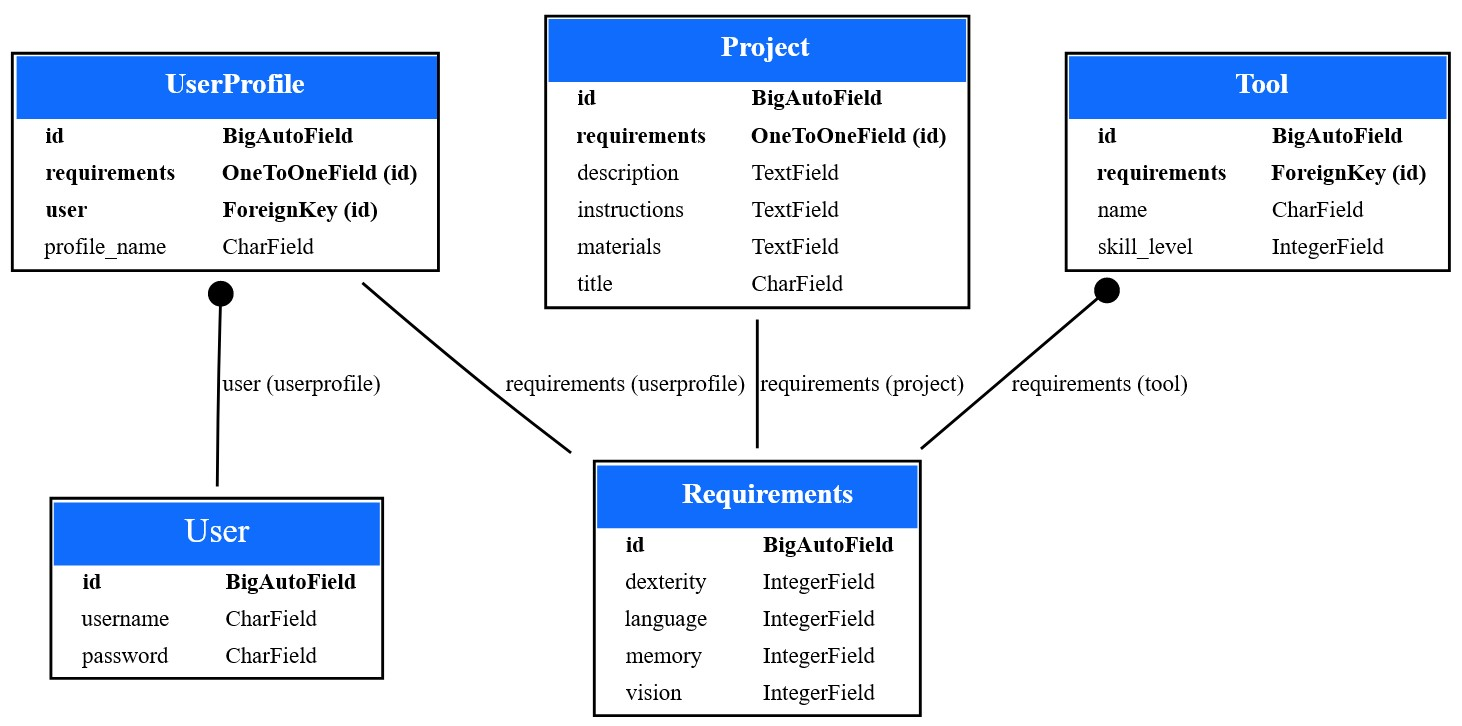
\includegraphics[width=\linewidth]{images/model.jpg}    

    \caption{Diagram of the Django models in Making Projects. One-to-many relationships are signified with a black circle. 
    }
    \label{fig:model_fig} 
\end{figure}

\section{Syllabus of Project Tutorials}
The syllabus creation algorithm is the core feature of the tool. It was implemented as a Django view function, which is Python code that is run when the user interacts with the syllabus creation page. It was redesigned several times in order to find a solution that worked well. We will outline the final implementation, along with the justification for several features which were shaped by our refactoring process. 

The algorithm consisted of several separate functions, in order to make it clearer and reuse code.

Firstly it requests the data it needs about the "end goal" project (end project). This calls a custom function of the Project model in order to only get the fields that are required. This function also collects all the related objects of the project, such as the skill area requirements and any physical tools that it uses. Originally this was done separately in the view function, but was redesigned to repeat less code and make more effective use of the database. An equivalent model function for the User Profile object is then called. 

Then it enters a while loop, which each time checks if the users profile is equivalent or greater than the end project, in terms of skill area levels. If they are not, it then calls a function that determines what areas the user still needs to improve which are returned as a list. 

This list is then passed into another function, along with the user's profile, which iterates through the list and queries the database for a project that matches the user profiles current values with that skill level incremented by one. Projects that contain tools that the user doesn't have access too, or not enough experience in, are not selected. If a project is not found on this first pass of the list, it reiterates through it but this time searches for projects with the incremented skill value, but accepts all other values that are equal to or less than the current user profile.  At first this constraint relaxing was not a feature, but was added in order to increase the chances of a syllabus being produced. We decided to keep it in conjunction with the first search function, as it would be more beneficial to a user to complete a project that better matches their requirements, if possible. 

Once a project is found, its information is appended to the syllabus, and the copy of the users profile is incremented accordingly. Then the while loop is ran again until the condition is met. 

Once this happens, the view function checks if the end project is in the syllabus and if not, appends it to the end. Then it calls the related model function on each project in the syllabus in order to get the information needed to display it for the user. This information is passed to the renderer, so that the user can see their syllabus. 


\section{Skill Area Requirements} 
The skill area requirements were implemented as a model, with the structure shown in figure \ref{fig:model_fig}. Originally skill area requirements were implemented as fields within their respective project or user profile objects. However we realised that these fields were repeated, and instead redesigned it as a separate model. This allowed for methods to be written that used this model, rather than having to repeat it for both the user profile and project models. 
This also allows for the possibility of having multiple requirements objects per project, which could then be used to adapt an individual project to a users needs as in requirement 
\textbf{FR-CH-8}. This was not implemented in this version of Making Projects, due to time constraints. 

Each skill area has three choices, which are the same for each skill but unique choices for each skill can easily be implemented without causing any loss of functionality.  

\subsection{Physical Tools}
The information about the physical tools were implemented as their own model. The ID of the related requirements object was stored as a field. This allowed for a one-to-many relationship between requirements and tools. Having them as separate objects made it simpler and more flexible when comparing the skill area requirements of user profiles and project tutorials. Users can only add tools to their profiles which are present in any of the project tutorials, this was implemented by creating a custom model manager that returns all distinct tool names present in the database and sets these values as the potential choices. Similarly, there is a constraint which prevents multiple tools with the same names being associated with one requirements object. They are four choices in what level of experience they have with that tool. Tool instances are deleted when their related requirements object is deleted.

\section{User Accounts}
The user accounts were implemented using Django's built in authentication system. This allowed us to utilise other features such as password hashing and validation functions. We chose to modify it to use the least amount of data as possible, in the form of a username and password. We opted to use an email instead of a traditional password, on the basis that it was more likely to be remembered. Despite it appearing as username in the code, due to Django requiring this, all forms were adapted to validate for an email address. 


\section{User Profiles}
We separated out user accounts and user profiles, as detailed in chapter \ref{design}. User profiles were implemented as a Django data model, which is then mapped to a relational database by Django's ORM. The user profile's requirements are stored as a separate data model, and linked to the profile. 

\subsection{Selection of User Profile}
Since it is possible for one user account to have multiple profiles, the tool had to be able to decide which profile to use at various points. To make it as consistent as possible, the profile which is to be used is stored as a session variable.  When a user logs in, if they only have one profile then it is automatically selected. If they have no profiles, the session variable is set to the value "None", and they are redirected to the "Create Profile" page. When a user has multiple profiles, their session variable is set to the value "None" and they are redirected to the "Select Profile" page so they can choose which profile they wish to use.
This page can also be used to switch which profile is the session variable at any point during the session. 

When a user creates a new profile, their session variable is set to that new profile. 
Session variables are deleted when the user logs out or when the browser is closed. This option can be toggled, and is currently set to delete on browser close to increase storage space and overall efficiency. However there is the consideration that it would be helpful for the end user to have their profile remain selected. 

\subsection{Updating User Profile} 
The user can update their details on the site. The page's template fetches their current details and displays them as the default values in the form so the user knows what their current values are. 

\section{Project Tutorials}
Similar in nature to the user profile, project tutorials were implemented as data models with related requirements models. All the functions surrounding them were stored within the data model, so that they were all in one place and could easily be used without rewriting code. 

It was important for the project tutorials to contain images. However instead of containing an absolute path to the images in the data model for each project, we created a function which dynamically looked up the file path based on a projects ID value and returned the images found in that directory. 

\section{General Site Appearance}
The appearance of the tool was a crucial consideration. It needed to be appealing as well as functional for people with many different abilities. We decided to use Bootstrap\footnote{https://getbootstrap.com/}, which is a front-end website toolkit, for the site's appearance. This allowed us to have an attractive looking website with minimal time spent on writing CSS. It also contains many of the best practices for web design, including some which we added, such as having hidden links for screen reader software to skip content, clearly naming all links, and using accurate alternative text for images. 

Django website pages are created using templates, which provided an ideal way to define a singular page design which could then be extended for each page leading to a consistent site design without repeating any code. The final design of the site can be seen in \ref{fig:syllabus}. 

\begin{figure}[htb]
    \centering
    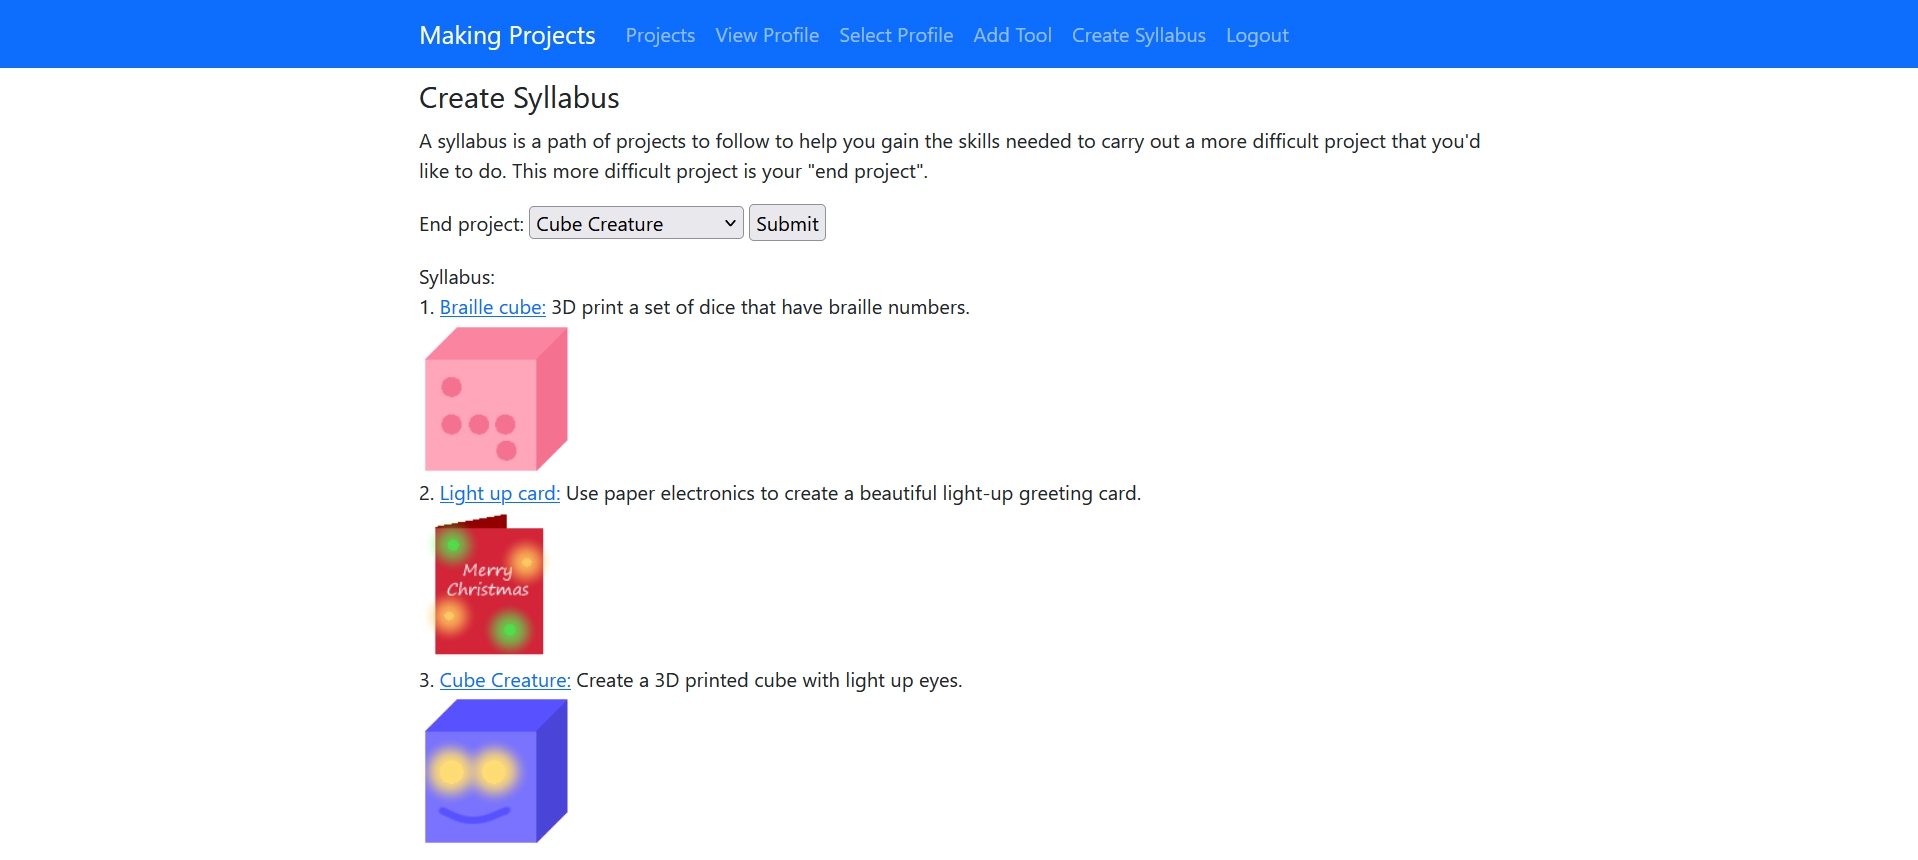
\includegraphics[width=\linewidth]{images/syllabus.png}    

    \caption{View of the syllabus page of Making Tools, showing the user interface design. 
    }
    \label{fig:syllabus} 
\end{figure}

\section{Admin Interface}
Django comes with a built in admin interface, which allows an admin user to interact with the database models through the site. We modified this to better suit the structure of our models and add additional functionality. As our tool used many related objects, one modification we made was displaying links to these objects when viewing said related object, as seen in \ref{fig:project_admin}. 

\begin{figure}[htb]
    \centering
    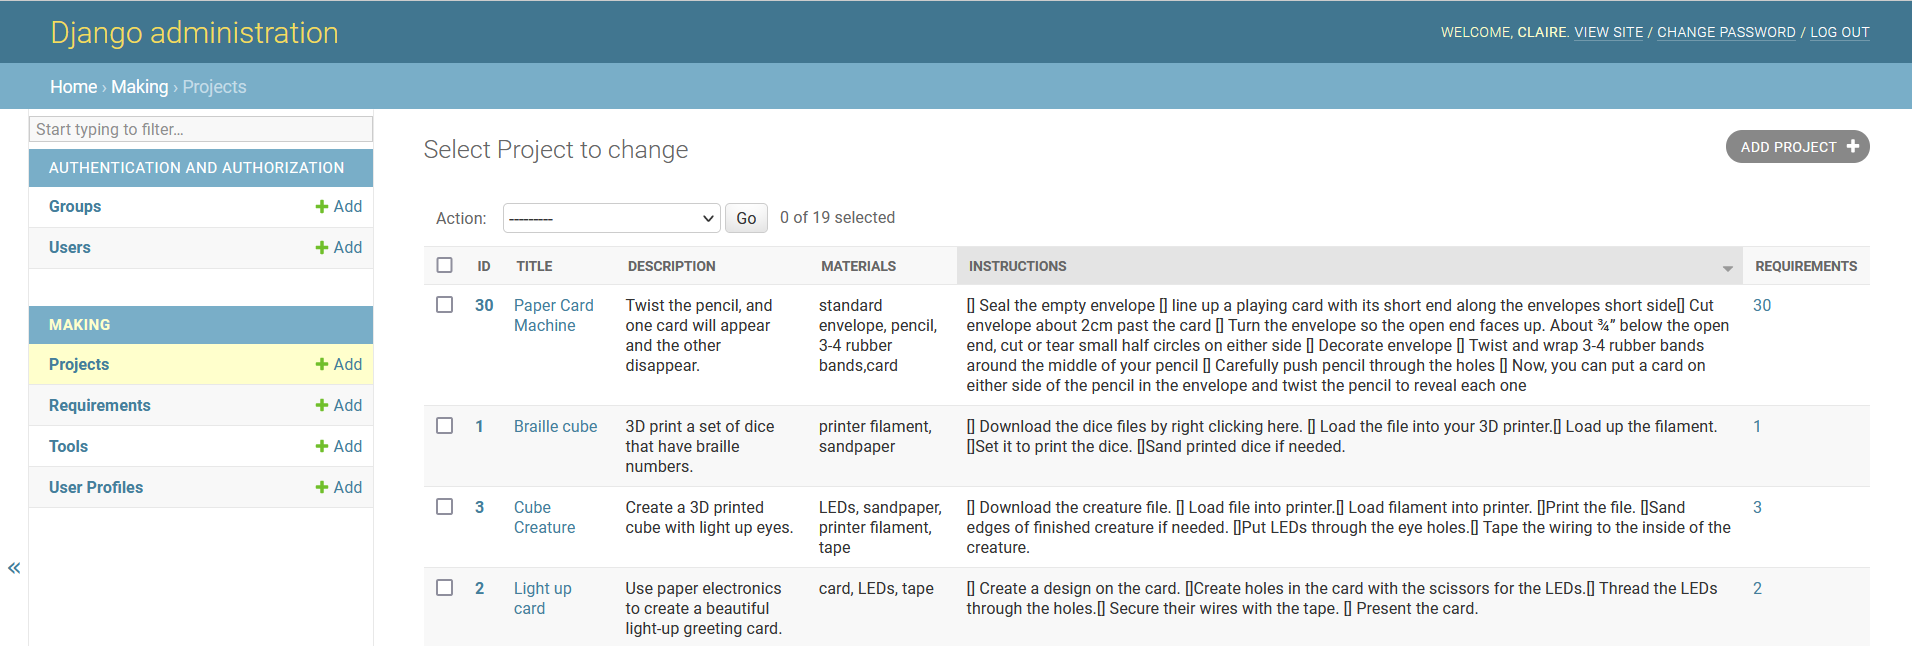
\includegraphics[width=\linewidth]{images/project_admin_2.png}    

    \caption{Image showing the admin view of project tutorials, displaying the links to their related requirements object.
    }
    \label{fig:project_admin} 
\end{figure}

We also added inline fields, which allowed a models related objects to be viewed and edited in the same place as the model. This can be seen in \ref{fig:related_tools}. This makes it easier to understand and work with the related data, while still allowing the actual models to be separate. 

\begin{figure}[htb]
    \centering
    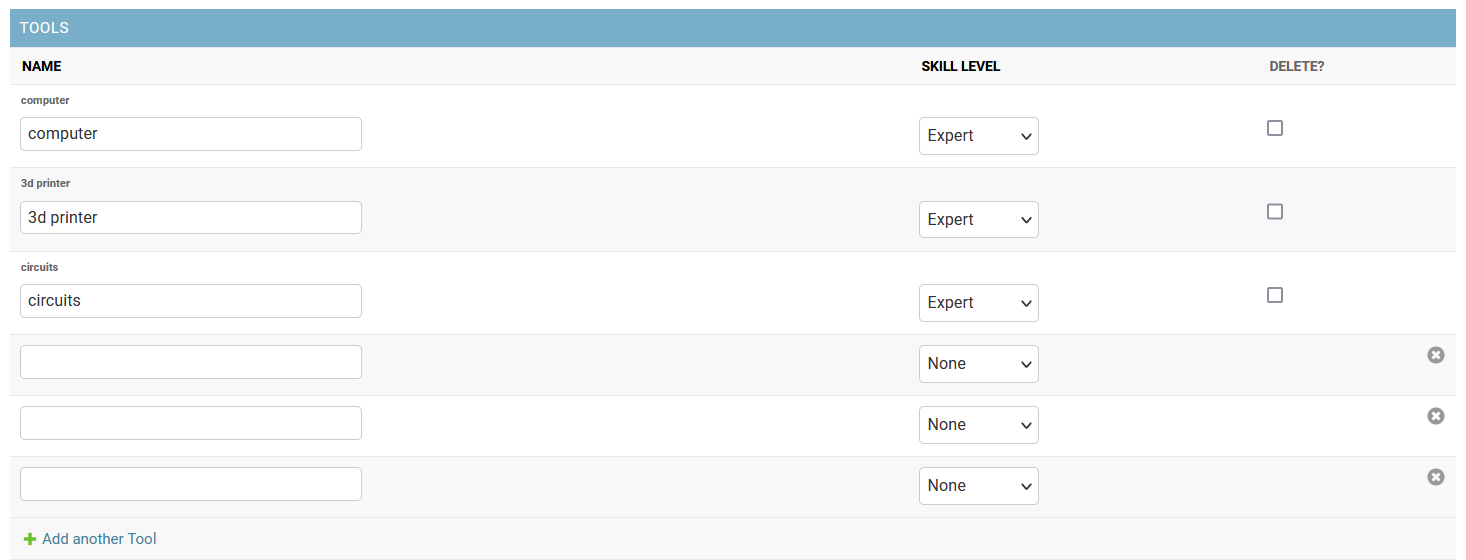
\includegraphics[width=0.75\linewidth]{images/related_tools.png}    

    \caption{Image showing the admin view of a requirements object, which shows its related tool objects and allows modification of them.
    }
    \label{fig:related_tools} 
\end{figure}

This was done to allow future developers, or other people using the tool, to easily modify the data without having to interact with the actual code. 
All of these changes were collected in one file that clearly labels the changes made. 


\noindent{\setlength{\fboxsep}{1em}\fbox{%
    \parbox{\textwidth-2em}{% 
        Now that Ruby has carried out a few projects with members of her group, she has a greater understanding of how the projects should be. She has found a project online that she would like to do with Cody, but would prefer to have it on Making Projects as he is used to using it. Since her organisation uses its own hosted version of Making Projects, she can log into it as an admin and easily add this new project, despite not having any knowledge of programming. 
    } % 
    }
} 

\section{Site Hosting}
The Django framework provides an ideal structure for web apps that can be easily hosted in different places. For this project, Making Projects was hosted using PythonAnywhere\footnote{https://eu.pythonanywhere.com/} which is a free to use Python development environment that allows hosting of Python projects.  
It was selected as it is low-cost and well suited for hosting Django projects, both in its capabilities and its resources on how to host a Django web app.  

However, Making Projects itself can readily hosted on a number of platforms. The code base contains clear instructions on how to do so, informed by the process of hosting on PythonAnywhere. This includes how to generate a secret key, and how to store it securely. 


%==================================================================================================================================
\chapter{Evaluation} 
\label{evaluation}
This chapter discusses the evaluation methods used for the tool, the results from those methods and their relation to the overall project requirements. We analyse these results in order to get an effective evaluation of Making Projects. 

Making Projects is designed to be used by people and so a user evaluation was important to understand how well the tool serves its purpose. 


\section{User Evaluation Experimental Design}
The user evaluation was run as a lab study due to it being an initial evaluation of the tool. We also did not have the time or resources to carry out an evaluation in a makerspace or disability support group. This is discussed in more detail within \ref{limitations} limitations.

Further evaluations outwith a lab study can benefit from the findings of this initial user evaluation. The results from this evaluation can also improve Making Projects before any more complex studies. 

The evaluation consisted of participants interacting with Making Projects with the experimenter observing. It conformed with every requirement from the University of Glasgow School of Computing Science ethics checklist, as shown in Appendix \ref{ethics-approval}. 

Participants were asked permission for an audio recording of the entire evaluation. The consent form can be seen at Appendix \ref{consent-form}. After written consent was given (no participant withheld permission), the audio recording was stored on a secure device, transcribed and rendered anonymous, and then all copies of the recording were deleted. 

One evaluation was carried out in person, and the other two through video calls and screen sharing. 


\subsection{Participants}
\label{participants}
The participants for the study all had knowledge of tangible learning and people with disabilities. We had approached participants for their knowledge in either area, but as it turned out they all had various degrees of experience in both. We classified knowledge of tangible learning as any involvement with makerspaces or similar organisations, or individual experience with hands on learning. Knowledge of people with disabilities included personal experience of having a disability, as well as working in roles that supported disabled people. 


\begin{table}[]
\centering
\caption{Overview of each participants demographics and experience in various areas.}
\label{tab:participant-profiles}
\begin{tabular}{lccllll}
\hline
\rowcolor[HTML]{E6E6E6} 
\textbf{ID} & \multicolumn{1}{l}{\cellcolor[HTML]{E6E6E6}\textbf{Gender}} & \multicolumn{1}{l}{\cellcolor[HTML]{E6E6E6}\textbf{Age}} & \textbf{Making} & \textbf{Makerspaces} & \multicolumn{2}{c}{\cellcolor[HTML]{E6E6E6}\textbf{Disability}} \\
\rowcolor[HTML]{E6E6E6} 
\textbf{}   & \multicolumn{1}{l}{\cellcolor[HTML]{E6E6E6}\textbf{}}       & \multicolumn{1}{l}{\cellcolor[HTML]{E6E6E6}\textbf{}}    & \textbf{}       & \textbf{}            & \textbf{Personal}            & \textbf{Professional}            \\ \hline
P1          & F                                                           & 18-25                                                       & High            & Moderate             & High                         & None                             \\
P2          & F                                                             & 18-25                                                         & Moderate        & None                 & High                         & Moderate                         \\
P3          & F                                                            & 18-25                                                         & High            & High                 & High                         & Moderate                         \\ \hline
\end{tabular}
\end{table}

\subsection{Pre-Study Interview}
Before each participant interacted with Making Projects, they had a semi-structured interview with the experimenter. The use of this structure allowed participants to share any information they fought relevant, while still covering all the same points in each interview. This interview lasted around 20 minutes and aimed to get an understanding of the participants experience with tangible learning, makerspaces, and people with disabilities. We also gathered demographic information in the form of their gender identity and age. 

\subsection{User Interaction with Making Projects}
Following the pre-study interview, participants where given access to Making Tools via a link to the hosted site on PythonAnywhere. This allowed participants to utilise any personalised adaptations they have made to their device, which is likely to occur in actual usage situations. This also allowed the site to be tested on multiple different types of device/screen.  
Participants were told to consider a potential user for Making Projects, and with that person in mind, carry out certain tasks. This was in order to evaluate the tool in relation to the intended end user, rather than the participant. The tasks were:
\begin{itemize}
    \item view a project tutorial
    \item register for an account
    \item enter their skill area requirements, and physical tools 
    \item select a suitable end goal project
    \item create a syllabus with that project
\end{itemize}
The observation allowed us to see how the participant navigated the site, and any issues they may have had.

\subsection{Post-Study Interview}
After using the tool, there was another interview with the participant. This was to gather their opinions of the tool. They were asked to identify any specific accessibility issues they noticed while using the tool, with the tool in general and also with the presentation of the project tutorials. Then they were asked which, if any, part of the tool they thought would be most useful in lowering the barriers to allow people with disabilities to carry out these projects. They were also invited to give any other opinions of the tool. 

\section{Limitations}
\label{limitations}
There were several limitations present in our user evaluation, and therefore our evaluation of Making Projects as a whole. 

While Making Projects is intended to be used by people with intellectual disabilities, involving these people in such a project requires a college level ethics approval application. This is a timely and complex process, with no guarantee of the application being approved, so the decision was made to not go ahead with it due to our limited time frame. However this did impact on our ability to fulfil requirement \textbf{NR-SH-16} as we could not interact with the intended end users. 

Instead, we reached out to local makerspaces and organisations which support people with intellectual disabilities. We introduced our project to them and asked if they would be willing to give their feedback on it and take part in an evaluation. We received encouraging responses from a few organisations, however when we attempted to arrange a follow up for an evaluation no organisations responded in time.  

Despite this, we remain hopeful that these organisations are amenable to be re-approached for future work in this area. 

In order to still carry out a meaningful evaluation of Making Projects, we then approached the people discussed in section \ref{participants}. This was not our ideal situation, but at this point our time frame was incredibly limited. 


\section{Analysis of User Evaluation}
Three main themes emerged from our analysis of the user evaluation results:  
\begin{itemize}
    \item[] \textbf{Removing Jargon} How the tool removed the need for knowledge of technical language, as well as areas where this could be improved. 
    \item[] \textbf{Legibility} The way in which the tool itself was accessible, and aspects which were not. 
    \item[] \textbf{Syllabus} How the syllabus worked and its perceived benefits to a user.
\end{itemize}
We will discuss each of them in more detail, and give an overall view of our findings from the evaluation.

\subsection{Removing Jargon}
All participants, to different extents, highlighted the use of plain non-technical language as beneficial to a potential user. They believed that this would lessen the amount of technical knowledge needed by a user to complete the projects.

Specific areas were identified as doing so, such as the explanations for skill levels and what each value meant. This was deemed particularly helpful to a potential user, as it effectively communicated what each option meant in a way which they could understand. One participant suggested that our choice of lesser known examples could hinder this, such as Duplo (a type of Lego block which is larger and easier to use), and that to aid understanding the tool could contain images of the objects given in the examples. We believe this to be a good idea, and have noted it in our areas for future work. 

One participant with less knowledge of tangible learning found the project tutorial instructions simple and easy to follow. They suggested that any acronyms be spelt out before being used, even ones we may consider basic or unneeded such as LEDs, in order to make the information more accessible to people with intellectual disabilities as well as screen reader technology. 

Another participant noted that displaying the skill level values as plain numbers across the tool was confusing as the context did not make it clear as to their meaning, and added an additional layer of complexity. Instead they suggested that we use relevant labels for the levels, rather than the raw numbers which is how they are stored in the database. We then implemented this, as these labels already existed for user input form and merely had not been extended across the tool. This allowed for a more cohesive and understandable design. We also made sure we were not using any similar numbers in other places of the tool, and instead using informative descriptors.  

\subsection{Legibility} 
A crucial point was that of having the tool be accessible and usable, in the context of people with intellectual disabilities. Participants views on this were shaped by their interactions with the tool as well as the points brought up by them in the interviews. 

Overall, the simple design of the user interface was described as beneficial by the participants as it made clear what a user could do and avoided confusion. However, all participants pointed out that the contrast between the navigation bar's background colour and its text was not high enough. This led to the text fading into the background slightly, which was noted as being a potential problem as it removed focus from the navigation bar. Additionally it could be difficult to read for people with visual impairments or issues with reading text. This can be changed in a future iteration of Making Projects to allow for a more effective and user friendly design. 

Another point raised was the significance of clearly showing the user the results of their actions. This was successful in some areas, such as the automatic redirection when a user created an account, and first line of text on the page visibly changing when a user switched profiles. One place where this was not successfully done however, was when the user created a new profile. Multiple participants noted that the current design did not make it obvious if the profile had been made or not, as the text indicating so blended in with the rest of the information. One participant took a while longer to realise it had been successful, whereas another participant did not see this text at all and instead created another profile. This problem can be addressed by putting more emphasis on any such text, and improving tolerance for error by giving users feedback on what has occurred in a way that they readily understand so they can respond accordingly. 

The use of external technology was also a discussion topic that came up in our interviews. It is likely that an intended end user has custom modifications to their technology which they wish to use when using Making Projects. These modifications aim to adapt the person's experience of using the technology in a way that is most accessible for their individual needs. Therefore it was important to the participants that both the external technology and Making Projects continue to function correctly when used together. This external technology could include software such as screen readers and display overlays, or hardware such as differently sized screens, and uncommon input devices. Two participants asked if the tool would work well with screen reader technology, and highlighted the importance of all links on the site being labelled correctly. 

While we had made a point to design the tool in a way that could be used by as many people as possible, we had not intended to comprehensibly evaluate the effects of different external technology on its functioning. However we were encouraged to discover that Making Projects could be used alongside one participants modifications, which included a "dark mode" plugin that altered the colours of the site, and a text highlighter and reader.  

\subsection{Syllabus} 
All participants were in agreement that the syllabus was the most helpful feature of the tool. They found the site's explanations of the syllabus and how to interact with it were intuitive, and did not require any further explanation from the experimenter. 

One participant discussed the importance of the syllabus, in that they believed it would allow a user to achieve their end goal. They had had the prior experience of wanting to be able to do something but not knowing how to get there, and were delighted by the prospect of being given a comprehensible list of projects. 

"If you're on your own and you know you want to achieve something but you're not sure how to get there, it will show you the intermediate steps."

Another point that was brought up was how the syllabus consisted of multiple, clearly defined "steps" (the projects). Participants agreed that this structure was beneficial in improving a persons knowledge, and allowing them to develop strategies for tangible learning. One participant added to this by sharing their lived experience of doing similar projects with a disability, and how a common pitfall was that they tried to do too much in too little time. They believed that this structure would help prevent this happening, by giving a user manageable tasks to complete separately. 

\section{Summary}
The user evaluation revealed problem areas of the tool which could then be addressed and improved. It also highlighted the importance of considering individual users needs, especially when designing for people with disabilities. As well as allowing us to gain a better understanding of how people would interact with the tool. We were satisfied that Making Projects met all its “must-have” functional and non-functional requirements.

%==================================================================================================================================
\chapter{Conclusion}    
In this chapter we will provide a summary of the entire project, along with our guidance for similar work, areas for future work that we have identified during this process, and a final reflection on this project as a whole. 

\section{Summary}
Tangible learning offers a fun alternative to traditional teaching methods. It has successfully been utilised by the maker movement to improve physical and abstract skills, create a community, and improve people's well being. However despite these benefits being well suited for people living with disabilities, especially intellectual disabilities, tangible learning as a whole remains inaccessible. Barriers such as physically demanding equipment and complex instructions prevent them from fully engaging with tangible learning. 

In order to facilitate tangible learning for people with disabilities, we proposed Making Projects, a tool which adapts project tutorials in a way that makes them easier to complete, and creates a customised syllabus of project tutorials. 

Making Projects uses the Django Python framework to create a modular and extensible web app that can leverage a users' needs to find a suitable course of projects. It can also calculate if a specific project is currently suitable for a user. 

We evaluated Making Projects with an user evaluation and found that it removed the need for complex technical language, was usable by people with different disabilities, and was effective in creating a syllabus of project tutorials. Combined, these findings shows that the tool is successful in lowering some of the barriers currently present in tangible learning. 

A hosted version of Making Projects can be found at ciw.eu.pythonanywhere.com. 


\section{Guidance for Similar Work}
Along with the areas outlined in section \ref{future-work}, the process of doing this project has revealed some aspects we believe that similar work could find helpful. 

Firstly, there should be a focus throughout the entirety of the project on involving the end user as much as possible. If this is not feasible, as in our case, then attempts should be made to involve people with experience of the end users. This will allow for an end product that is more suited for its purpose and therefore more efficient. 

When creating something to be used by people with disabilities, it should allow for as much customisation as possible. While we were aware of this from researching Universal Design \citep{Cen1997}, it was not made apparent until the user evaluation the sheer degree of customisation that can be beneficial to a user. 


\section{Future Work}
\label{future-work}
During the course of this project we have identified potential areas for future work, both to improve Making Projects, and for the general research field of improving people with disabilities access to tangible learning. Some of these areas are requirements from chapter \ref{requirements-analysis} that we did not have enough time to fulfil. 

\subsection{Physical Projects}
Making Projects focused more on creating an environment to facilitate tangible learning, rather than the tangible learning projects themselves. Therefore future work on what tangible learning projects are most suitable, and how to overcome common accessibility issues with them, is vital in allowing more people with disabilities to access tangible learning.   

\textbf{DIY-AT} In addition to this, project tutorials that result in a piece of assistive technology (AT) was a requirement of this project (\textbf{FR-CH-9}) which we did not have the time to complete. However it is still a relevant area which could provide great benefit for people with disabilities, both in their tangible learning processes and day to day life.

\subsection{Optimisation of Syllabus Creation}
In its current form, the syllabus creation algorithm is sufficient. However it is inefficient as in the worst case, it requires multiple searches of all the projects in the database. This will be exacerbated as more projects are added to the tool. Therefore it would be beneficial to optimise this process. This could be done by sorting the database, or refactoring the algorithm to require less searches. 

Changes could also be made with the order in which skill areas are chosen for improvement. At the moment, skill areas are improved first if a suitable project exists, before any physical tools. This feature could be modified in conjunction with user evaluation of the specific projects in a syllabus, to result in a syllabus that is most effective in teaching a user. 

\subsection{Additional Features for Making Projects}
There are many features that could improve Making Projects, several of which are discussed below. These were either requirements that did not have time to be implemented, or which were made apparent during the user evaluation of the tool. 

\textbf{Record of project completion} Allowing users to see what projects they have previously completed was a requirement (\textbf{FR-SH-6}) that did not manage to get implemented. It was independently brought up by participants during the evaluation as a good potential feature to have. Making Projects having this would allow users to feel a sense of achievement, as well as not requiring users to recall what projects they have already done. This is relevant as people with intellectual disabilities often have impeded memory.

\textbf{Project Tutorial Filtering} Being able to find a project that you want, and are able, to do is a process integral to Making Projects. However the users experience of this could be further improved, as made apparent during the user evaluation. Features such as a search engine that returns projects with a certain skill level, for example low dexterity, could allow users to see their options for project tutorials. An indication of the skill level needed on the tutorial previews could also improve this. This could be in the form  of small simple icons representing each skill, with the number of icons representing how much experience in that skill is needed. 


\section{Final Reflection} 
This project has taught me a lot about how to manage and organise a large piece of work, especially its importance when the overall time frame is limited. 
I also learnt how crucial it is to follow best practices when designing a software system, particularly when considering modularity. It became even more clear after my understanding of the project developed and I attempted to add new features to my original design, only to have to redesign the entire structure. In retrospect, using a database engine that allowed for greater filtering of queries such as PostgreSQL would have allowed for greater extensibility for features such as a search engine for project tutorials. SQLite is lightweight but at the cost of having less functionality. 
The process of evaluating this project has allowed me to understand just how important user evaluations are for a tool like this, in order to gain awareness of how effective the tool is in its intended environment. 
Finally, the process of writing this paper has taught me valuable skills in how to effectively convey the purpose and development of my project through academic writing. 

%==================================================================================================================================
%
% 
%==================================================================================================================================
%  APPENDICES  

\begin{appendices}

\chapter{Appendices}


\pdfsection{Ethics Approval}{images/ethics_checklist.pdf}
\label{ethics-approval}

\pdfpage{Evaluation Consent Form}{images/consent_form.pdf}
\label{consent-form}

\pdfpage{Evaluation Introduction Script}{images/evaluation_intro.pdf}
\label{eval-intro}

\pdfpage{Information on Making Projects for User Evaluation}{images/evaluation_info.pdf}
\label{eval-info}

\pdfpage{Evaluation Debriefing Script}{images/debriefing_info.pdf}
\label{eval-debrief}

\section{Outline of Source Code}
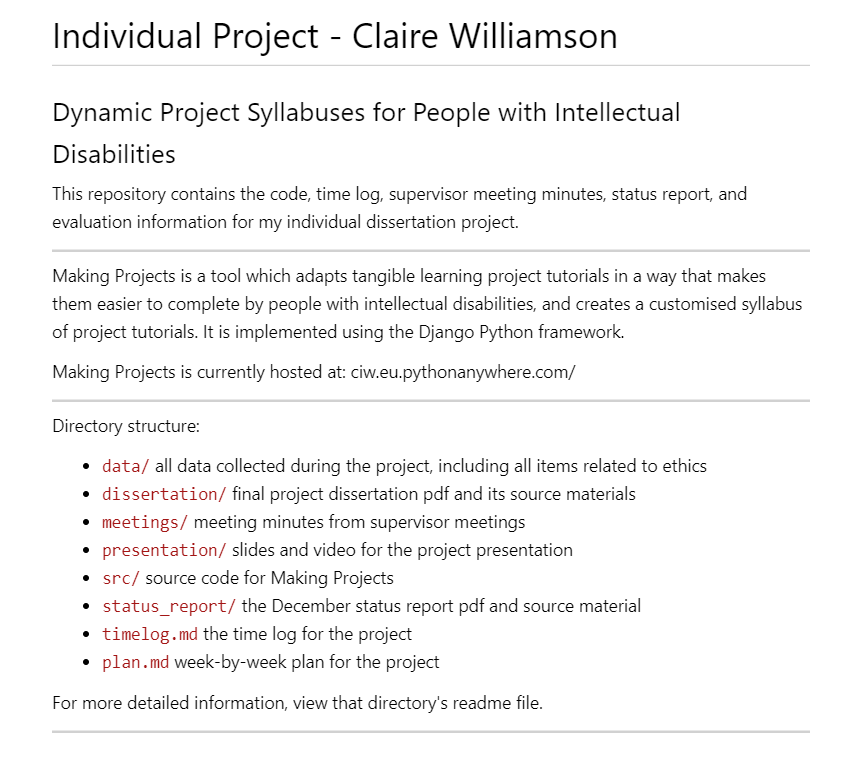
\includegraphics[width=0.75\linewidth]{images/readme1.png}  
\section{User Manual}
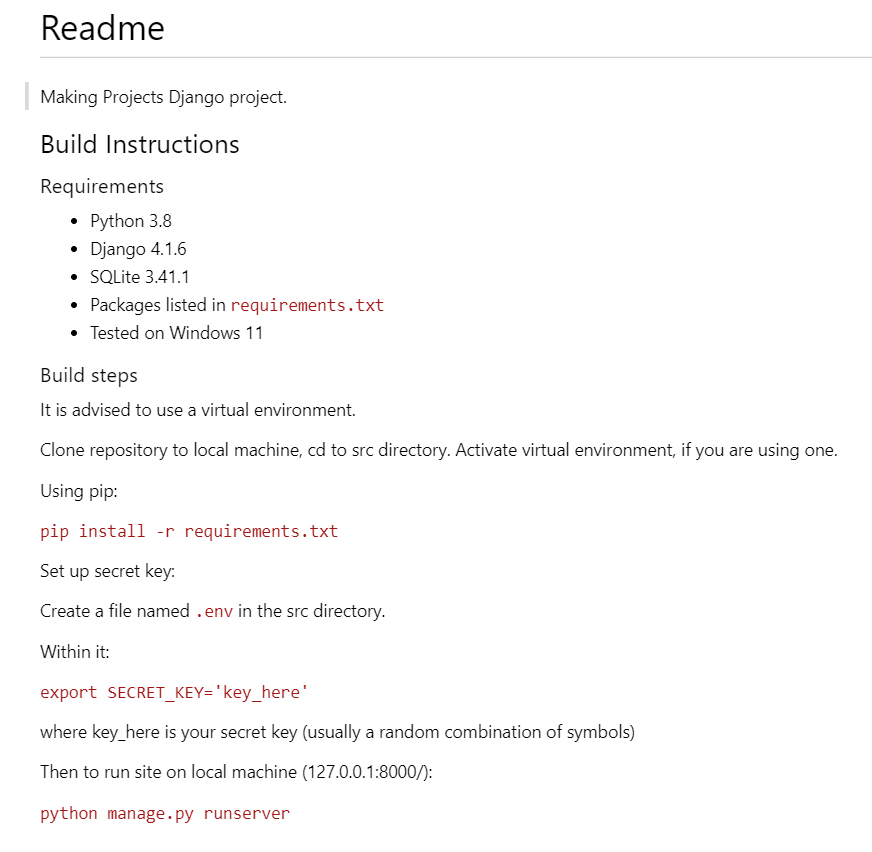
\includegraphics[width=0.75\linewidth]{images/readme.png}  


\end{appendices}

%==================================================================================================================================
%   BIBLIOGRAPHY   

% The bibliography style is abbrvnat
% The bibliography always appears last, after the appendices.

\bibliographystyle{agsm}
\renewcommand{\thechapter}{0} 
\bibliography{l4proj}

\end{document}
